\documentclass[slidestop,compress,mathserif,note=show, blackandwhite]{beamer}
%% [slidestop] puts frame titles on the top left corner
%% (default=[slidescentered]).
%% [compress] makes all navigation bars as small as possible
%% (default=[uncompressed]).
%% [red] changes navigation bars and titles to reddish color.


% for bold faced structures (titles, headlines, footlines, sidebars, ...)
\usefonttheme{structurebold}
\usepackage{euler}
\usepackage{graphics}
\usepackage{wrapfig}
\mode<presentation> 

%% \usepackage{ragged2e}
%% \justifying

\setbeamercovered{transparent} 
\definecolor{myYellow}{RGB}{252,187,6}

%hideallsubsections, hideothersubsections 
\usetheme[left, hideothersubsections ]{Goettingen}                  % Beamer theme v 3.0
\usecolortheme{crane}                % Beamer color theme

\setbeamercolor{title}{fg=blue}
\setbeamercolor{subtitle}{fg=black}
\setbeamercolor{frametitle}{fg=black}
\setbeamercolor{section in sidebar}{fg=black, bg=myYellow}
\setbeamercolor{section in sidebar shaded}{fg=blue}
\setbeamercolor{subsection in sidebar}{fg=black, bg=myYellow}
\setbeamercolor{subsection in sidebar shaded}{fg=black}

% general data
\title [R.E.A.R.] {Rear Exocentric Augmented Reality}
\subtitle []{an exocentric vision framework for mobile robot teleoperations}
\author []{Daniele Ferro}
\date []{March 28, 2011}
\institute [UniCT] {Universit\`a di Catania\\Dipartimento di Ingegneria Elettrica Elettronica e Informatica [DIEEI]}

\begin{document}

% Cover slide
\begin{frame}    
 \titlepage
\end{frame}

% slide indice
\section[Outline]{}
%\tiny
\frame{

  \frametitle{Outline}
  \tableofcontents[pausesections]
}
\small

%% INTRODUCTION

\section{Introduction}
\section{Introduction}
\label{sec:intro}

\section{Virtual Presence and Telerobotics}
\label{intro:virtual_presence}

Man has always dreamt of being able to be present in more than
one place at the same time.
\\
In Hindu Mythology all the gods had multiple avatars, which
allowed them to exist in multiple domains simultaneously and to
serve the purpose of representing the original in different
places. In this way, gods could accomplished more useful work
at the same time. 
\\
This dream has always been one of the aims to achieve for 
researchers and industries. With the advent of Internet and
advanced computer and electronic technologies, we can get a
step closer to obtain presence in more than one place
at a time.
\\
What we need is the equivalent of a body in the remote environment,
with which we can move around, perform the proper actions through,
and observe with. By combining elements of Internet and
telerobotics it is possible to transparently immerse users into
navigable real remote worlds and to make such systems accessible
from any networked computer in the world. In essence, we obtain
\textit{Virtual Presence}.
\\
Virtual Presence removes the barriers of distance and offers a
reasonable facsimile of instantaneous travel to anywhere on earth
from any networked computer.
In Virtual Presence we have a telerobot which provides a form
(a physical avatar) that can be moved round in a remote space.
A telerobot is a robot that accepts instructions from a distance,
generally from a trained human operator. The human operator thus
performs live actions in a distant environment and through sensors
can gauge the consequences.
\\
The telerobot is hence equipped with a web-camera, laser scanning and
others type of sensors (see chapter \ref{intro:3morduc} for \morduc{}
concrete example). All these devices are used to provide the
necessary feedback for an effective feel of the remote domain.
\\
More formally, telerobotic is based on two main concepts, referred to
as \textit{teleoperation} and \textit{telepresence}.
\\
Teleoperation means `doing work at a distance', although `work' may
mean almost anything. The term `distance' is also vague: it can refer
to a physical distance, where the operator is separated from the robot
by a large distance, but it can also refer to a change in scale, where
for example in robotic surgery a surgeon may use micro-manipulator
technology to conduct surgery on a microscopic level.
\\
Telepresence means `feeling like you are somewhere else'.
Thus a user, sitting at a remote computer far away from the target
domain, can comfortably roam about, observe and even command
specific action to be performed in the vicinity of the telerobot.
\\
There are many jobs which a human could perform better than a robot, but
for some reasons humans either do not want to or can not perform it.
The job may be too dangerous, for example exploring inside a volcano;
other jobs must instead be executed in location physically inaccessible.
For example, exploring another planet, inspecting areas with very high
level of radiations, cleaning the inside of a long pipe or performing
laparoscopic surgery.
\\
Looking at these new perspectives robots are going to be more complex
than factories ones, built and programmed to accomplish few repetitive
tasks. Different kind of operations are not easy
to automate, and nowadays it is hard to develop autonomous robots, so
it is necessary to drive them by teleoperation and virtual reality.
\\
Looking back in history, some of our most influential technologies
- such as the telescope,
telephone, and television - were developed to provide knowledge
at a distance. Telerobotic systems date back to the need for handling
radioactive materials in the 1940s, and in the 1950's they were developed
to facilitate action at a distance. Remote controlled robot are now
being applied to exploration, bomb disposal, and surgery.
\\
Specialists use telerobots to actively explore environments such
as Mars and Chernobyl, while military personnel increasingly employ
reconnaissance drones and telerobotic missiles.
In the summer of 1997, the film Titanic included scenes with undersea
telerobots and NASA's Mars Sojourner telerobot successfully
completed a mission on Mars.
\begin{figure}
  \begin{center}
    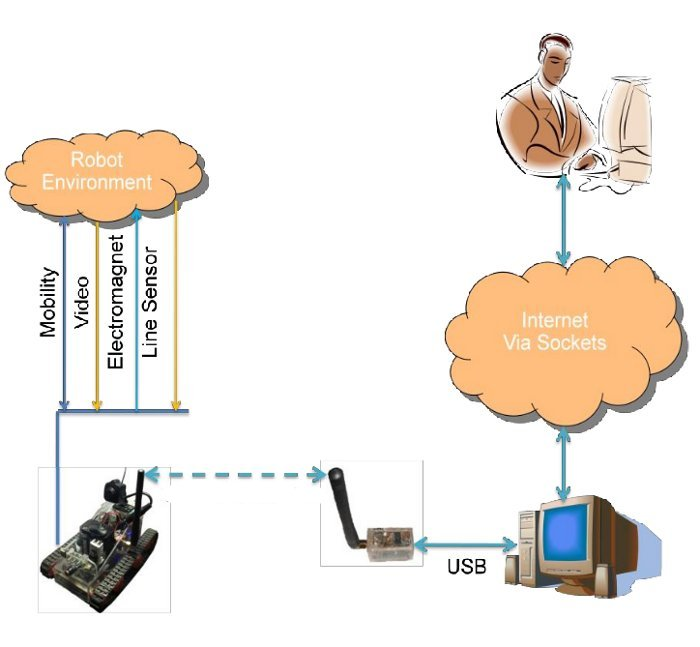
\includegraphics[width=270pt]{img/user_robot_inter.jpg}
    \caption{Generic Interaction human-robot through Internet}
    \label{fig:user_robot_inter}
  \end{center}
\end{figure}
\\
The Internet dramatically extends our scope and reach, since we can simply
teleguide the robot from any part of the world. The bidirectional
structure of the Internet offers furthermore a new means for actions:
through one communication channel telerobotic device can send data
collected by its sensors to the operator, in order to fulfil the
illusion of being in the remote place and to have a robust feedback;
on the other channel the operator can send the proper commands to
be performed by the robot. Illustration \ref{fig:user_robot_inter}
gives a graphical example.

\newpage
\section{Mobile robot}
\label{intro:mobile}

Mobile robots (or telerobot) have the capability to move around
in their environment and are not fixed to one physical location.
\\
As stated in \cite{robot:whereami}, Leonard and Durrant-Whyte
(in 1991) summarized the general problem of mobile robot navigation
by three questions:

\begin{itemize}
\item \texttt{Where am I ?}
\item \texttt{Where am I going ?}
\item \texttt{How should I get there ?}
\end{itemize}

This section surveys the some basic notions in sensors 
and technologies that aim at answering the
first question.
\\
We will often refer to the expression \textit{robot navigation},
that is primarily about guiding a mobile robot to a desired destination
or along a pre-specified path. For these reasons teleoperator must
be able, with an as great as possible precision, to know the robot's
position in its environment, which consists of landmarks and obstacles.
\\
In order to achieve this objective the robot needs to be equipped with
sensors suitable to localise the robot throughout the path it is to follow.
These sensors may give overlapping or complementary information and may
also sometimes be redundant. Because of the lack of a single, generally
good method, developers of  automated guided vehicles (AGVs) and mobile
robots usually combine two or more methods to localize the robot.
\\
All these sensor measurements can be fused to estimate the robot's
position by using a sensor fusion algorithm. Sensor fusion
in this case is the method of integrating data from distinctly
different sensors to estimate the robot's position.
\\
The sensors used to localize the mobile robot can be categorized into
two groups: internal and external sensors. The ones belonging to the first
group measure some internal state of the robot, such as motion, acceleration,
direction.
\\
Sensors belonging to the second group (external sensors) provide information
about objects in the workspace surrounding the robot.
\\
Sensors that will be exposed in this section are:
\begin{itemize}
\item \texttt{Encoder} \\
  Internal sensor, details in chapter \ref{intro:mobile:encoder}
\item \texttt{Laser} \\
  External sensor, details in chapter \ref{intro:mobile:laser}
\item \texttt{Sonar} \\
  External sensor, details in chapter \ref{intro:mobile:sonar}
\item \texttt{Bumper} \\
  External sensor, details in chapter \ref{intro:mobile:bumper}
\item \texttt{Image sensor} \\
  External sensor, details in chapter \ref{intro:mobile:image}
\end{itemize}

Data collected with previous sensors must be processed with proper methods to
determinate robot's position. Among these we will briefly cite: 
\begin{itemize}
\item \texttt{Odometry} \\
  Details in chapter \ref{intro:mobile:odometry}
\item \texttt{Inertial Navigation} \\
  Details in chapter \ref{intro:mobile:inertial}
\item \texttt{Video based positioning} \\
  Details in chapter \ref{intro:mobile:video}
\end{itemize}

%%------------------------------------------------------------------

\subsection{Encoder}
\label{intro:mobile:encoder}

The simplest type of incremental encoder is a single-channel
\textit{tachometer encoder}, basically an instrumented mechanical
light chopper that produces a certain number of sine or square wave
pulses for each shaft revolution. Adding pulses increases the resolution
(and subsequently the cost) of the unit.
\begin{figure} [h]
  \begin{center}
    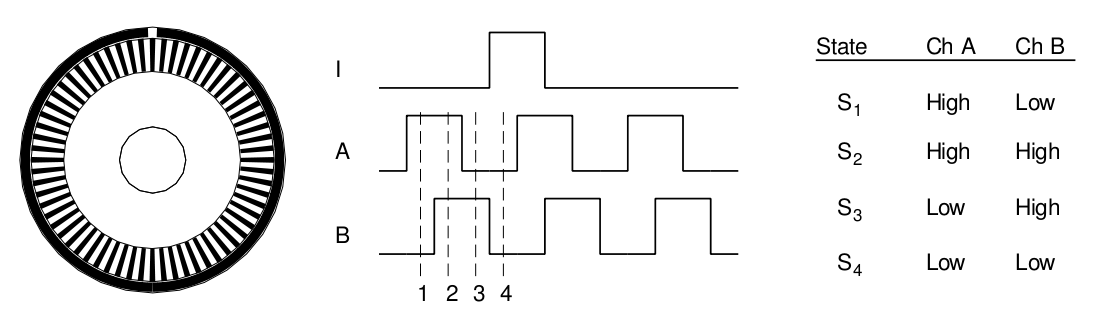
\includegraphics[width=\textwidth]{img/incremental_encoder.png}
    \caption{The observed phase relationship between Channel A and B
      pulse trains can be used to determine
      the direction of rotation with a phase-quadrature encoder,
      while unique output states S1 - S4 allow for up to a
      four-fold increase in resolution. The single slot in the outer
      track generates one index pulse per disk rotation.
    }
    \label{fig:incremental_encoder}
  \end{center}
\end{figure}
\\
These relatively inexpensive devices are well suited as velocity feedback
sensors in medium to high speed control systems, but run into noise and
stability problems at extremely slow velocities due to quantization errors.
\\
The tradeoff here is resolution versus update rate: improved transient
response requires a faster update rate, which for a given line count reduces
the number of possible encoder pulses per sampling interval. 
\\
In addition to low-speed instabilities, single-channel tachometer encoders
are also incapable of detecting the direction of rotation and thus cannot
be used as position sensors. Phase-quadrature incremental encoders overcome
these problems by adding a second channel, displaced from the
first, so the resulting pulse trains are 90 degrees out of phase, as shown
in figure \ref{fig:incremental_encoder}.
\\
This technique allows the decoding electronics to determine which channel
is leading the other and hence ascertain the direction of rotation, with the
added benefit of increased resolution.
\\
The incremental nature of the phase-quadrature output signals dictates that
any resolution of angular position can only be relative to some specific
reference, as opposed to absolute. Establishing such a reference can be
accomplished in a number of ways. For applications involving continuous
360-degree rotation, most encoders incorporate as a third channel a special
index output that goes high once for each complete revolution of the shaft
(see figure \ref{fig:incremental_encoder}).
\\
Intermediate shaft positions are then specified by the number of encoder
up counts or down counts from this known index position.
\\
One disadvantage of this approach is that all relative position information
is lost in the event of a power interruption.
\\
Interfacing an incremental encoder to a computer is not a trivial task.
A simple state-based interface as implied in Figure 1.1 is inaccurate if
the encoder changes direction at certain positions, and false pulses can
result from the interpretation of the sequence of state changes.
\begin{figure} [!h]
  \begin{center}
    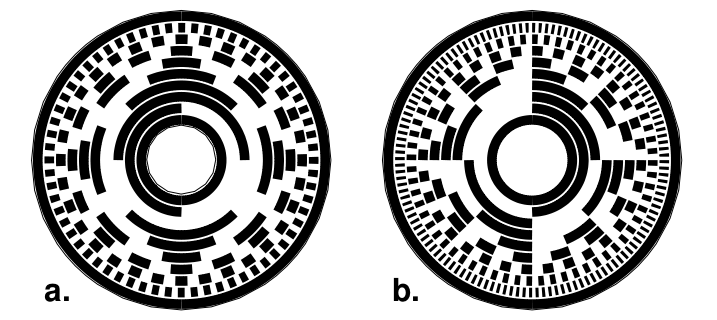
\includegraphics[width=300pt]{img/absolute_encoder.png}
    \caption{Rotating an 8-bit absolute Gray code disk.
      a. Counterclockwise rotation by one position increment will cause
      only one bit to change.
      b. The same rotation of a binary-coded disk will cause all bits to
      change in the particular case (255 to 0) illustrated by the
      reference line at 12 o'clock.}
    \label{fig:absolute_encoder}
  \end{center}
\end{figure}
\\
Absolute encoders are typically used for slower rotational applications
that require positional information when potential loss of reference
from power interruption cannot be tolerated.
\\
Instead of the serial bit streams of incremental designs, absolute optical
encoders provide a parallel word output with a unique code pattern for each
quantized shaft position. The most common coding schemes are \textit{Gray code},
natural binary, and binary-coded decimal.
\\
The Gray code (for inventor Frank Gray of Bell Labs) is characterised by the
fact that only one bit changes at a time, a decided advantage in eliminating
asynchronous ambiguities caused by electronic and mechanical component tolerances
(see figure \ref{fig:absolute_encoder}a).
\\
Binary code, on the other hand, routinely involves multiple bit changes when
incrementing or decrementing the count by one. For example, when going from
position 255 to position 0 in figure \ref{fig:absolute_encoder}b, eight
bits toggle from 1s to 0s. Since
there is no guarantee all threshold detectors monitoring the detector elements
tracking each bit will toggle at the same precise instant, considerable ambiguity
can exist during state transition with a coding scheme of this form.
\\
Some type of handshake line signaling valid data available would be required
if more than one bit were allowed to change between consecutive encoder positions.
\\
Absolute encoders are best suited for slow and/or infrequent rotations such
as steering angle encoding, as opposed to measuring high-speed continuous
(i.e., drive wheel) rotations as would be required for calculating displacement
along the path of travel.
\\
A potential disadvantage of absolute encoders is their parallel data output,
which requires a more complex interface due to the large number of electrical leads.


\subsection{Laser}
\label{intro:mobile:laser}

In laser-based systems, also known as \textit{laser radar} or
\textit{lidar}, a beam of light is emitted in a rapid sequence
of short bursts aimed directly at the object being ranged.
\\
The time required for a given pulse to reflect off the object
and return is measured and used to calculate distance to the
target based on the speed of light. Accuracies for early sensors
of this type could approach a few centimeters over the range
of 1 to 5 meters.
\\
The method above is also used in ultrasonic sensors (we refer to
chapter \ref{intro:mobile:sonar} for more details), where sound pulses
are transmitted and the reflection time is measured (also known as
\textit{time of flight} or shortly \textit{TOF}).
\\
The TOF is directly proportional to the distance between the scanner
and the object. By indicating with \textit{L} the distance between
the laser and the obstacle, whereas with \textit{c} the light speed,
the formula to reckon up TOF is:

\[
t_{flight} = \frac{2L}{c}  \Longrightarrow  L = \frac{t_{flight}}{2}\cdot c
\]

The quality of time of flight range sensors manly depends on:

\begin{itemize}
\item Uncertainties about the exact time of arrival of the reflected signal
\item Inaccuracies in the time of fight measure
\item Interaction with the target (surface, specular reflections)
\item Variation of propagation speed
\item Speed of mobile robot and target
\end{itemize}

\begin{figure} [h]
  \begin{center}
    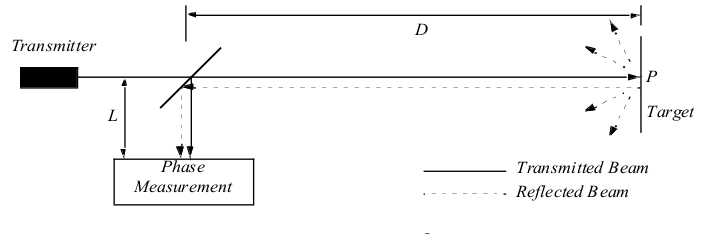
\includegraphics[width=\textwidth]{img/laser_shift_phase.png}
    \caption{Phase-Shift Measurement}
    \label{fig:laser_shift_phase}
  \end{center}
\end{figure}

Another easier method, working with laser beams, is to transmit 100\%
amplitude modulated light beam at a defined frequency and compare
the phase shift between the transmitted and the reflected light (a scheme
is presented in figure \ref{fig:laser_shift_phase}).
\\
This scanner has much higher resolution. The mathematical formulas to
obtain distance follow. We indicate with \textit{f} the modulating
frequency; with \textit{c}, once again, the light speed. We can calculate
the wavelength \textit{$\lambda$} as:

\[
\lambda = \frac{f}{c}
\]

The distance covered by the emitted light, \textit{D'}, referring to
the distances \textit{D} and \textit{L} showed in figure
\ref{fig:laser_shift_phase}, is equal to:

\[
D' = L + 2 \cdot D = L + \frac{\theta}{2\cdot\pi}\cdot\lambda
\]

where \textit{$\theta$} is the phase difference between transmitted
and reflected beacon, return by the module `phase measurement'.
In the end, distance \textit{D} is reckoned by the following formula:

\[
D = \frac{\lambda}{4\cdot\pi}\cdot{\theta}
\]

Confidence in the range (phase estimate) is inversely proportion to
the square of the received signal amplitude.
\begin{figure} [h]
  \begin{center}
    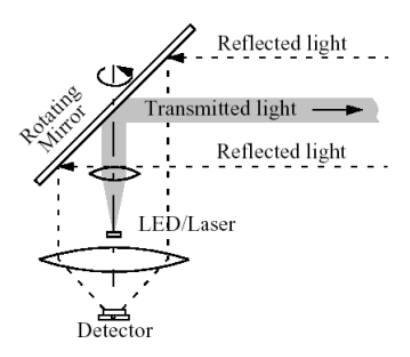
\includegraphics[width=200pt]{img/laser_rotation.png}
    \caption{Schematic drawing of laser range sensor with
      rotation mirror.}
    \label{fig:laser_rotation}
  \end{center}
\end{figure}
\\
Pointing the measuring beam
to rotating mirror a fast scanning can be accomplished in a vertical
dimension, but the whole scanner has to be able to move horizontally
if 3D scanning is needed. A schematic drawing for 2D scanner laser
is showed in figure \ref{fig:laser_rotation}.
\begin{figure} [!h]
  \begin{center}
    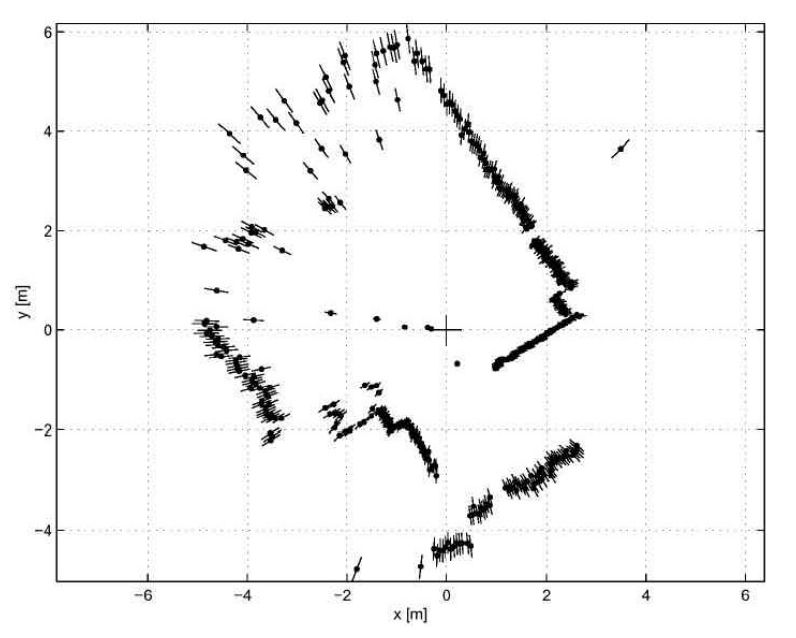
\includegraphics[width=250pt]{img/laser_scan_map.png}
    \caption{Typical range image of a 2D laser range sensor with a
      rotating mirror.}
    \label{fig:laser_scan_map}
  \end{center}
\end{figure}
\\
In figure \ref{fig:laser_scan_map} a typical range image of a 2D
laser range sensor with
a rotating mirror is shown. The lengths of the lines through the
measurement points indicate the uncertainties.


\subsection{Sonar}
\label{intro:mobile:sonar}

Ultrasonic TOF ranging is today the most common technique employed
on indoor mobile robotics systems, primarily due to the ready
availability of low-cost systems and their ease of interface.

Active sonar creates an ultrasonic pulse, often called `ping',
then listens for reflections `echo'. Referring to figure
\ref{fig:sonar}, the ping wave is drawn in red, the echo wave
in green.
\begin{figure} [h]
  \begin{center}
    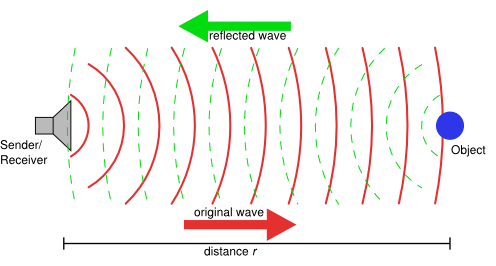
\includegraphics[width=300pt]{img/sonar.png}
    \caption{Sonars in action}
    \label{fig:sonar}
  \end{center}
\end{figure}
\\
The received signal is commonly processed by measuring the time of flight,
already explained in previous section (\ref{intro:mobile:laser}).
This time is depending on the speed of the sound in air, and thus the
temperature, humidity, air pressure, and so on may effect measurements.
\\
The knowledge of time of flight enables the computation of the distance
to the target, which reflected the pulse.
\\
The sonar field of view is a cone and the sensitive area increases
proportionately with the distance. It is necessary to introduce an
inhibition time to avoid the false obstacles due to the ping signal.
On the other hand, the inhibition time does not allow reading
distance too short.
\\
The main drawback with the sonar sensor is its wide beam of perception, which
causes the fact that it is impossible from reading returned data to identify
the object position within the beam. Some of the other sonar drawback are
specular reflection and the possibility of a crosstalk.
\begin{figure} [!h]
  \begin{center}
    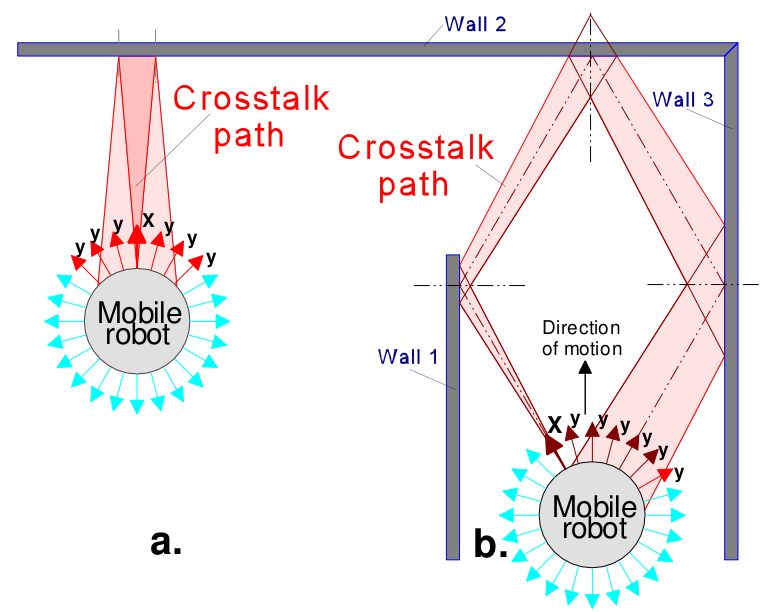
\includegraphics[width=250pt]{img/sonar_crosstalk.png}
    \caption{Example of crosstalk effects with sonar sensors.}
    \label{fig:sonar_crosstalk}
  \end{center}
\end{figure}
\\
Figure \ref{fig:sonar_crosstalk} shows an example of crosstalk.
Crosstalk is a phenomenon in which one sonar picks up the echo
from another. One can distinguish between a. direct effectiveness
of ultrasonic sensors in crosstalk and b. indirect crosstalk.


\subsection{Bumper}
\label{intro:mobile:bumper}

The basic explanation given for why mobile robots need instrumented
bumpers is for a last line of defense type of sensor, one that takes
over if the IR (infra-red), sonar, or other navigational sensors fail
to detect an obstacle. Or, more bluntly, if your other sensors misses
an obstacle, the bumper will indicate the robot has impacted with an
object of unknown size and shape. The robot then can initiate some
sort of evasive/escape maneuvers to
hopefully get back on track to its destination.
\begin{figure} [!h]
  \begin{center}
    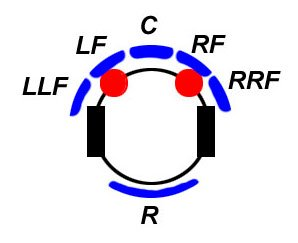
\includegraphics[width=200px]{img/bumpers.jpg}
    \caption{A robot provided with five bumpers, four on front
      side and one on rear side.}
    \label{fig:bumpers}
  \end{center}
\end{figure}
\\
Another advantage of using bumpers is that the impacts derived from
collisions are cushioned, avoiding seriously damages to the robot's
instruments.

\subsection{Image sensors}
\label{intro:mobile:image}

An image sensor is a device that converts an optical image to an electric
signal; it is used mostly in digital cameras and other imaging devices.
\\
Early sensors were video camera tubes but a modern one is typically a
charge-coupled device (also known as \textit{CCD}) or a complementary
metal-oxid-semiconductor (\textit{CMOS}) active pixel sensor.
\\
Today, most digital still cameras use either a CCD image sensor or a
CMOS sensor. Both types of sensor accomplish the same task of capturing
light and converting it into electrical signals.
\\
A CCD is an analog device. When light strikes the chip it is held as a small
electrical charge in each photo sensor. The charges are converted to voltage
one pixel at a time as they are read from the chip. Additional circuitry in
the camera converts the voltage into digital information.
\\
A CMOS chip is a type of active pixel sensor made using the CMOS semiconductor
process. Extra circuitry next to each photo sensor converts the light
energy to a voltage; additional circuitry on the chip may be included
to convert the voltage to digital data.
\begin{figure} [!h]
  \begin{center}
    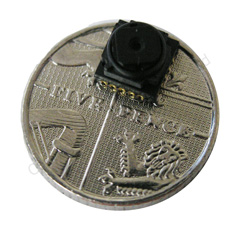
\includegraphics[width=100pt]{img/cmos_camera.jpg}
    \caption{A CMOS camera.}
    \label{fig:cmos_camera}
  \end{center}
\end{figure}
\\
Neither technology has a clear advantage in image quality. On one hand,
CCD sensors are more susceptible to vertical smear from bright light sources
when the sensor is overloaded.
CMOS can potentially be implemented with fewer components, use less power,
and/or provide faster readout than CCDs.
CMOS sensors are less expensive to manufacture than CCD sensors.
\\
There are many parameters that can be used to evaluate the performance
of an image sensor, including its dynamic range, its signal-to-noise ratio,
its low-light sensitivity, etc. For sensors of comparable types,
the signal-to-noise ratio and dynamic range improve as the size increases.
\\
For more details see \cite{wiki:image_sensor}.

\subsection{Odometry}
\label{intro:mobile:odometry}

Odometry is the most widely used navigation method for mobile robot
positioning. It is well known that odometry provides good short-term
accuracy, is inexpensive, and allows very high sampling rates. However,
the fundamental idea of odometry is the integration of incremental motion
information over time, which leads inevitably to the accumulation of errors.
\\
Particularly, the accumulation of orientation errors will cause large
position errors which increase proportionally with the distance traveled
by the robot. Despite these limitations, most researchers agree that odometry
is an important part of a robot navigation system and that navigation tasks
will be simplified if odometric accuracy can be improved. Odometry is used
in almost all mobile robots, for various reasons:

\begin{itemize}
\item odometry data can be fused with absolute
  position measurements to provide better and more
  reliable position estimation;
\item odometry can be used in between absolute position updates with
  landmarks. Given a required positioning accuracy, increased accuracy
  in odometry allows for less frequent absolute position updates. As
  a result, fewer landmarks are needed for a given travel distance;
\item many mapping and landmark matching algorithms assume that the robot
  can maintain its position well enough to allow the robot to look for
  landmarks in a limited area;
\item in some cases, odometry is the only navigation information available.
  For example when no external reference is available, when circumstances
  preclude the placing or selection of landmarks in the environment,
  or when another sensor subsystem fails to provide usable data.
\end{itemize}

Odometry is based on simple equations, depending on mobility configuration
chosen for the robot, that are easily implemented and that utilise
data from inexpensive incremental wheel encoders.
\begin{figure} [!h]
  \begin{center}
    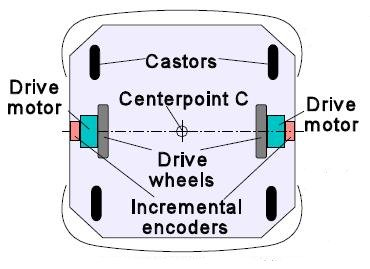
\includegraphics[width=200pt]{img/differential_drive.jpg}
    \caption{A CMOS camera.}
    \label{fig:differential_drive}
  \end{center}
\end{figure}
\\
In \textit{differential-drive}, one of the available robot configuration
shown in figure \ref{fig:differential_drive}, incremental encoders
are mounted onto the two
drive motors to count the wheel revolutions.
\\
The robot can compute, by simple geometric equations, the momentary
position of the vehicle relative to a known starting position.
\\
Suppose that at sampling interval \textit{i} the left and right wheel
encoders show a pulse increment of \textit{$N_{L,i}$} and \textit{$N_{R,i}$},
respectively. Suppose further that

\[
c_m = \frac{\pi \cdot D_n } {n \cdot C_e }
\]

where

\textit{$c_m$} = conversion factor that translates encoder pulses into
linear wheel displacement \\
\textit{$D_n$} = nominal wheel diameter (in mm) \\
\textit{$C_e$} = encoder resolution (in pulses per revolution) \\
\textit{n}   = gear ratio of the reduction gear between the motor
(where the encoder is attached) and the drive wheel \\
\\
we can compute the incremental travel distance for the left and
right wheel, $\bigtriangleup$$U_{L,i}$ and $\bigtriangleup$$U_{R,i}$,
according to

\[
\bigtriangleup U_{L,i} = c_m \cdot N_{L,i}
\]
\[
\bigtriangleup U_{R,i} = c_m \cdot N_{R,i}
\]

and the incremental linear displacement of the robot's centerpoint
\textit{C}, denoted $\bigtriangleup$$U_{i}$, according to

\[
\bigtriangleup U_{i} =
\frac{{\bigtriangleup U_{L,i}} + {\bigtriangleup U_{R,i}}} {2}
\]

Next, we compute the robot's incremental change of orientation

\[
\bigtriangleup \theta_i =
\frac{{\bigtriangleup U_{R,i}} - {\bigtriangleup U_{L,i}}} {b}
\]

where \textit{b} is the wheelbase of the vehicle, ideally measured
as the distance between the two contact points between the wheels
and the floor.
\\
The robot's new relative orientation $\theta_i$ can be computed from
\[
\theta_i = \theta_{i-1} + \bigtriangleup \theta_i
\]

and the relative position of the centerpoint is

\[
x_i = x_{i-1} + \bigtriangleup U_{i} \cdot \cos \theta_i
\]
\[
y_i = y_{i-1} + \bigtriangleup U_{i} \cdot \sin \theta_i
\]

where
\\
\textit{$x_i$}, \textit{$y_i$} = relative position of the
robot's centerpoint \textit{C} at instant i-th.
\\
Unfortunately, odometry is
based on the assumption that wheel revolutions can be translated
into linear displacement relative to the floor.
\\
This assumption is only of limited validity. One extreme example is
wheel slippage: if one wheel was to slip on, say, an oil spill, then
the associated encoder would register wheel revolutions even though
these revolutions would not correspond to a linear displacement of the
wheel.
\\
Along with the extreme case of total slippage, there are several other
more subtle reasons for inaccuracies in the translation of wheel encoder
readings into linear motion. All of these error sources fit into one
of two categories: systematic errors and non-systematic errors.
Systematic errors include:

\begin{itemize}
\item unequal wheel diameters
\item average of actual wheel diameters differs from 
  nominal wheel diameter
\item actual wheelbase differs from nominal wheelbase
\item misalignment of wheels
\item finite encoder resolution
\item finite encoder sampling rate
\end{itemize}

Non-systematic errors include:

\begin{itemize}
\item travel over uneven floors.
\item travel over unexpected objects on the floor.
\item Wheel-slippage due to slippery floors, over-acceleration,
  fast turning (skidding), external or internal forces, non-point wheel
  contact with the floor.
\end{itemize}

The clear distinction between systematic and non-systematic errors is
of great importance for the effective reduction of odometry errors. For example,
systematic errors are particularly grave because they accumulate constantly.
On most smooth indoor surfaces systematic errors contribute much
more to odometry errors than non-systematic errors.
However, on rough surfaces with significant irregularities, non-systematic
errors are dominant.
\begin{figure} [h]
  \begin{center}
    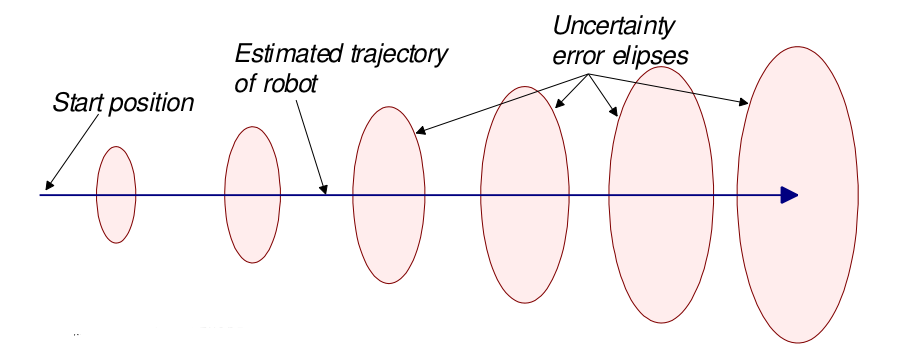
\includegraphics[width=310pt]{img/odometry_error.png}
    \caption{Growing `error ellipses' indicate the growing position
      uncertainty with odometry.}
    \label{fig:odometry_error}
  \end{center}
\end{figure}
\\
The problem with non-systematic errors is that they may appear unexpectedly
(for example, when the robot traverses an unexpected object on the
ground), and they can cause large position errors. Typically, when a mobile
robot system is installed with a hybrid odometry/landmark navigation system,
the frequency of the landmarks is determined
empirically and is based on the worst-case systematic errors. Such systems
are likely to fail when one or more large non-systematic errors occur.
\\
It is noteworthy that many researchers develop algorithms that estimate
the position uncertainty of a robot. With this approach each computed robot
position is surrounded by a characteristic `error ellipse', which
indicates a region of uncertainty for the robot's actual position (see
figure \ref{fig:odometry_error}).
\\
Typically, these ellipses grow with travel distance, until an absolute
position measurement reduces the growing uncertainty and thereby `resets'
the size of the error ellipse.

\subsection{Inertial navigation}
\label{intro:mobile:inertial}

An alternative method for enhancing dead reckoning is
inertial navigation, initially developed for deployment on
aircraft.
\\
The principle of operation involves continuous sensing of minute
accelerations in each of the three directional axes and integrating over time
to derive velocity and position. A gyroscopically stabilized
sensor platform is used to maintain consistent orientation of the three
accelerometers throughout this process.
\\
Although fairly simple in concept, the specifics of implementation are
rather demanding. This is mainly caused by error sources that adversely
affect the stability of the gyros used.
\\
Experimental results indicate that a purely inertial navigation approach
is not realistically advantageous (i.e., too expensive) for mobile robot
applications.
\\
Inertial navigation is attractive mainly because it is self-contained
and no external motion information is needed for positioning. One important
advantage of inertial navigation is its ability to provide fast, low-latency
dynamic measurements.
\\
Furthermore, inertial navigation sensors typically have noise and error sources
that are independent from the external sensors. For example, the noise and error
from an inertial navigation system should be quite different
from that of, say, a landmark-based system.
\\
Fundamentally, gyros provide angular rate and accelerometers provide
velocity rate (i.e. acceleration) information. Dynamic information is
provided through direct
measurements. However, the main disadvantage is that the angular rate data
and the linear velocity rate data must be integrated once and twice (respectively),
to provide orientation and linear position, respectively.
\\
Thus, even very small errors in the rate information can cause an unbounded
growth in the error of integrated measurements.

\subsection{Video based positioning}
\label{intro:mobile:video}

A core problem in robotics is the determination of the position and
orientation of a mobile robot in its environment. The basic principles
of landmark-based and map-based positioning also apply to the vision-based
positioning or localization which relies on optical sensors
in contrast to ultrasound, laser and inertial sensors.
Common optical sensors include cameras using CCD arrays.
\\
Visual sensing provides a tremendous amount of information about a
robot's environment, and it is potentially the most powerful source of
information among all the sensors used on robots.
\\
Due to the wealth of information, however, extraction of visual features
for positioning is not an easy task. The problem of localization by vision has
received considerable attention and many techniques have been suggested.
The basic components of the localization process are:

\begin{itemize}
\item representations of the environment
\item sensing models
\item localization algorithms
\end{itemize}

Most localization techniques provide absolute or relative position and/or
the orientation. Techniques vary substantially, depending on the sensors,
their geometric models, and the representation of the environment.
\\
The geometric information about the environment can be given in the form
of landmarks, object models and maps in two or three dimensions. A vision
sensor or multiple vision sensors should capture image features or regions
that match the landmarks or maps.
\\
On the other hand, landmarks, object models, and maps should provide necessary
spatial information that is easy to be sensed. When landmarks or maps of an
environment are not available, landmark selection and map building should
be part of a localization method.
\\
Geometric models of photometric cameras are of critical importance for
finding geometric position and orientation of the sensors. The most common
model for photometric cameras is the pin-hole camera with perspective projection
as shown in figure \ref{fig:camera_system}. Photometric cameras using optical lens can
be modeled as a pin-hole camera.
\begin{figure} [h]
  \begin{center}
    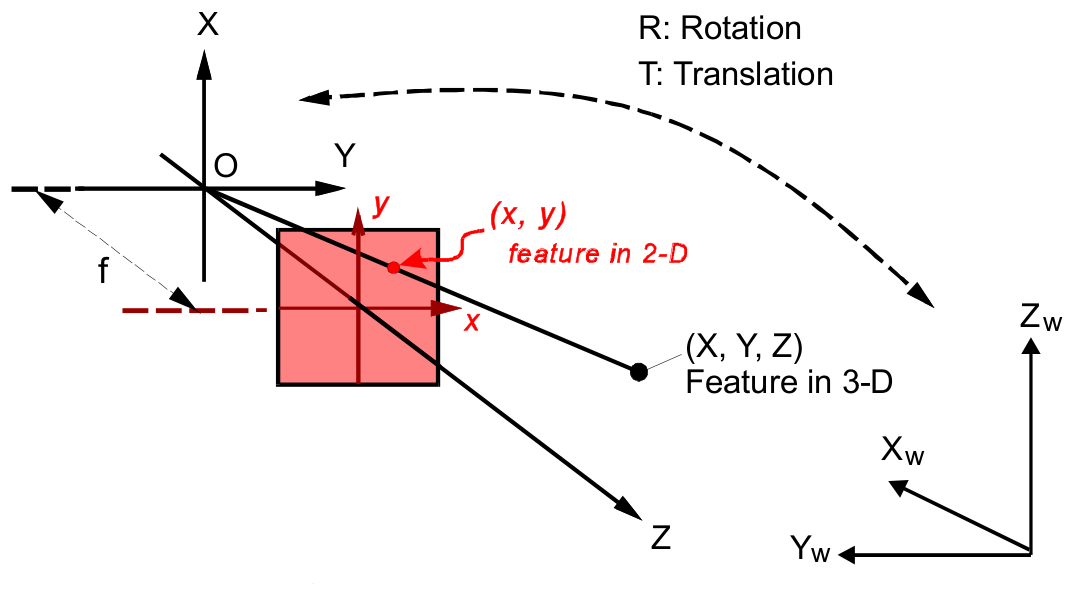
\includegraphics[width=350pt]{img/camera_system.png}
    \caption{Perspective camera model.}
    \label{fig:camera_system}
  \end{center}
\end{figure}
\\
The coordinate system (X, Y, Z) is a three-dimensional camera coordinate
system, and (x, y) is a sensor (image) coordinate system. A three-dimensional
feature in an object is projected onto the image plane (x, y). The relationship
for this perspective projection is given by

\[
x = f \cdot \frac{X}{Z}
\]

\[
y = f \cdot \frac{Y}{Z}
\]

where \textit{f} is the distance the two systems' origins.
\\
Although the range information is collapsed in this projection, the angle or
orientation of the object point can be obtained if the focal length \textit{f}
is known and there is no distortion of rays due to lens distortion.
\\
The internal parameters of the camera are called `intrinsic camera parameters' and
they include the effective focal length f, the radial lens distortion factor,
and the image scanning parameters, which are used for estimating the physical
size of the image plane.
\\
The orientation and position of the camera coordinate system (X, Y, Z) can be
described by six parameters, three for orientation and three for position, and
they are called `extrinsic camera parameters'. They represent the relationship
between the camera coordinates (X, Y, Z) and the world or object coordinates
(XW, YW, ZW).
\\
Landmarks and maps are usually represented in the world coordinate system.
The problem of localization is to determine the position and orientation of a
sensor (or a mobile robot) by matching the sensed visual features in one or
more image(s) to the object features provided by landmarks or maps. Obviously a
single feature would not provide enough information for position
and orientation, so multiple features are required.
\\
Depending on the sensors, the sensing schemes, and the representations of the
environment, localization techniques vary significantly.

\newpage
\subsection{The 3morduc platform}
\label{sec:3morduc}

\begin{figure} [h]
  \begin{center}
    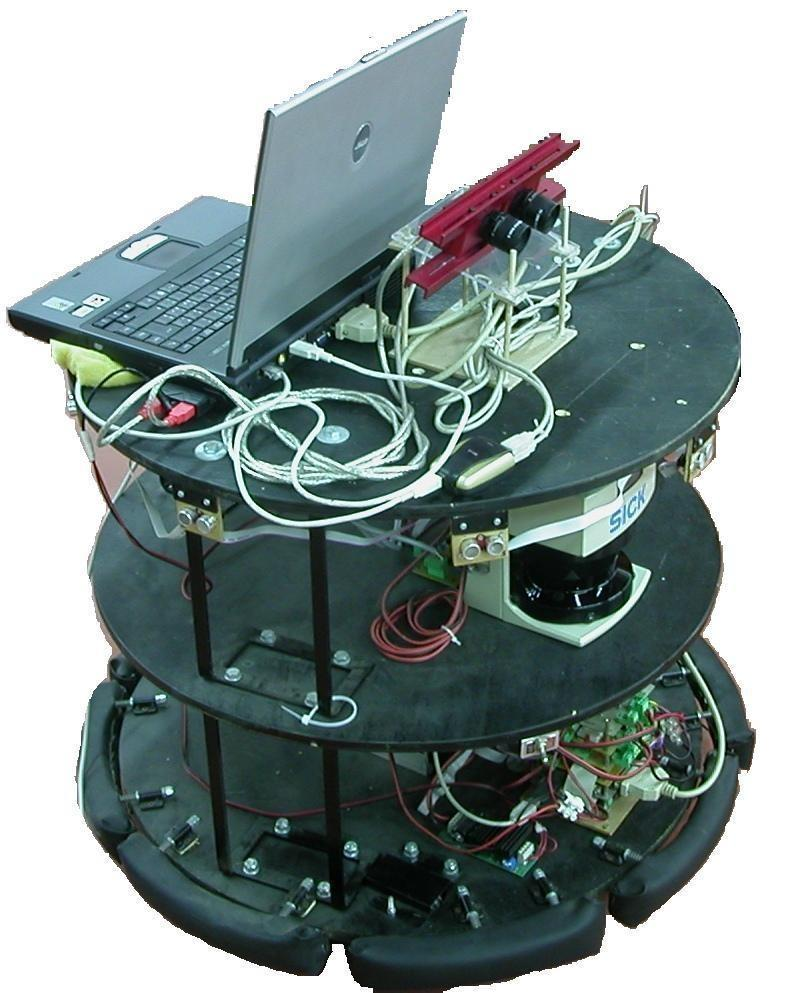
\includegraphics[width=150pt]{img/3morduc.jpg}
    \caption{The 3morduc robotic platform}
    \label{fig:morduc}
  \end{center}
\end{figure}

The telerobot used to develop teleoperation research is
called \textit{3MO.R.D.U.C.}, acronym for `3rd version of
the Mobile Robot DIEES University of Catania'.
3morduc is a mobile-robot, able to move forward, backward
and turn its direction, as directed by the remote operator.
It has been successfully used in several test and experimental
work regarding teleoperation and telepresence.
\\
The robot, actually located at the University of
Catania, is a differential-driven mobile robot, showed
in figure \ref{fig:morduc}.
\\
As every mobile robot, it is equipped with some internal
and external sensors, through which is possible retrieve
information about, respectively, the status of the robot
(e.g. its position) or the data about the environment (e.g.
distance from obstacles).

\subsubsection{Sensors and actuators}
\label{sec:3morduc:sensors_actuators}


The movement is performed by means of two 40W DC engines, model
\textit{Maxon F2260}, connected with the motor shaft by a gear
box (transmission rate 1/19). On the other side the motor shaft
is linked with two rubber wheels, while a third castor wheel can
freely turn to realize the differential-driven model.
\\
The robot is compound by three shelves, each one connected to
the next. On the lower level two lead batteries are situated,
able to erogate 12 Volts at 18 Amperes. The electrical autonomy is
granted for 30-40 minutes.
\begin{figure}[h]
  \begin{center}
    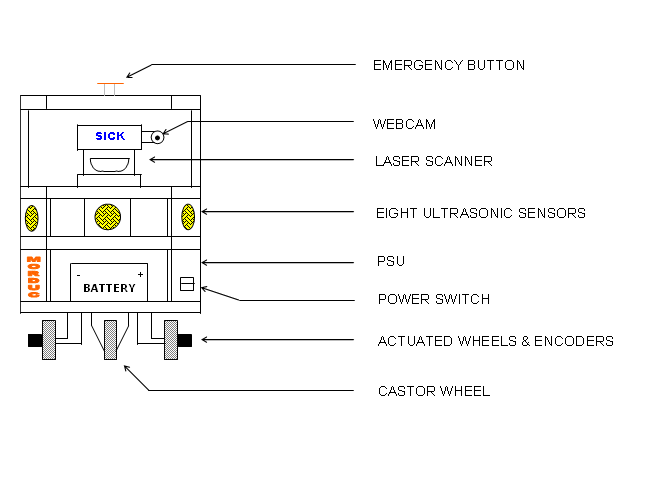
\includegraphics[width=300pt]{img/Morduc_scheme.png}
    \caption{3morduc's schematic figure}
    \label{fig:morduc_scheme}
  \end{center}
\end{figure}
\\
Besides, on the same lower level is located an electronic board
controlling different modules, each one predisposed to manage a
specific task as movements, sensors and communication.
\\
Type and number of sensors available on 3morduc are:

\begin{itemize}
\item \texttt{belt of bumpers} \\
  A belt of bumpers (in total 16 switches) is dislocated around
  the entire perimeter on the robot base, just over the wheels level. \\
  See chapter \textit{Bumper} (\ref{sec:mobile:bumper}) for more details
  about this type of sensor.

\item \texttt{incremental encoders} \\
  The two robot motor axes are equipped with incremental encoders, with
  resolution of 500 pulses per turn. These sensors are useful to calculate
  heading and position of the robot by using the kinematic model. \\  
  See chapter \textit{Encoder} (\ref{sec:mobile:encoder}) for more details
  about this type of sensor.
 
\item \texttt{belt of sonars} \\
  On the second level are located eight sonar sensors, which measure the
  distance from an obstacle using the flight time of an ultrasonic signal
  produced by means of a vibrating piezoelectric sensor. \\
  See chapter \textit{Sonar} (\ref{sec:mobile:sonar}) for more details
  about this type of sensor.

\item \texttt{scanner laser} \\
  In order to detect obstacles on the workspace, the \textit{Laser Measurement
  Sensor} (LMS) operates by measuring the flight time of a pulsed laser
  light beam that is reflected by obstacle, to provide a 2D scanning data. \\
  It is possible to configure different angular resolution (0.25\textdegree,
  0.5\textdegree or 1\textdegree pace) with different angular scan (100\textdegree
  or 180\textdegree).
  \begin{figure}[h]
    \begin{center}
      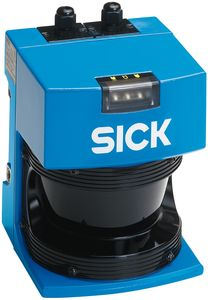
\includegraphics[width=60pt]{img/laser_sick_lms_200.jpg}
      \caption{LMS Sick mounted on 3morduc}
      \label{fig:laser_sick_lms_200}
    \end{center}
  \end{figure}
  \\
  See chapter \textit{Laser} (\ref{sec:mobile:laser}) for more details
  about this type of sensor. The reference manual about \textit{LMS
  Sick 200} can be found at \cite{3morduc:laser_sick_200}.

\item \texttt{stereo cameras} \\
  On the robot there are also two stereoscopic cameras, each one with a
  resolution of 1.3 megapixel and fixed focus lens of 4.0 mm. \\
  The CCD sensors of these cameras have a good noise immunity and
  sensibility; moreover, it is possible to adjust all the image parameter, e.g.
  exposure gain, frame rate, resolution. \\
  The cameras are mounted on a rigid support; it permits to simply adjust
  the camera distance in a range 5-20 cm. \\
  Both the cameras can be connected to PC by IEEE 1394 interface, with a
  frequency of synchronization of 8 KHz. \\
  \begin{figure}[h]
    \begin{center}
      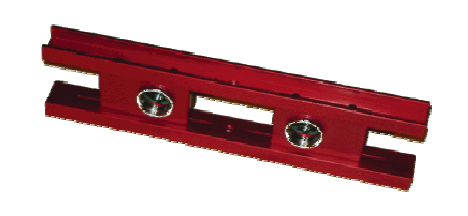
\includegraphics[width=200pt]{img/camera_videre.png}
      \caption{STH-MDCS2-VAR-C mounted on 3morduc}
      \label{fig:camera_videre}
    \end{center}
  \end{figure}
  \\
  See chapter \textit{Image sensors} (\ref{sec:mobile:image}) for more details
  about this type of sensor. The reference manual about the \textit{STH-MDCS2-VAR-C}
  can be found at \cite{3morduc:camera_sth_mdcs2}.

  

\end{itemize}

More images, video and information about 3morduc can
be found at \cite{morduc:features}.


\subsubsection{Internet communication}
\label{sec:3morduc:communication}

The network system implemented on the 3morduc is a typical
client-server architecture: in order to control the robot through
Internet, 3morduc implements an HTTP server.
\\
Through different type of prearranged HTTP requests, a generic
HTTP client sends command to the server and retrieve information
about 3morduc's status. In this way, client needs only to open a TCP/IP
socket on the HTTP standard port (number 80) to control the robot from
remote.
\begin{figure}[h]
  \begin{center}
    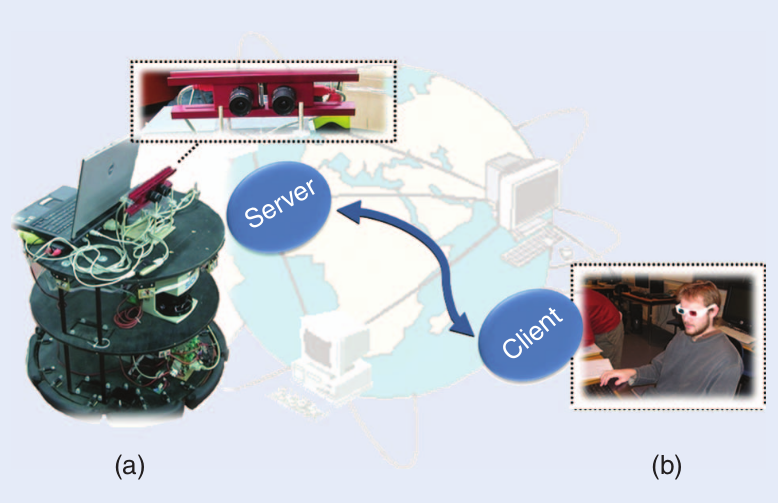
\includegraphics[width=300pt]{img/3morduc_client_server.png}
    \caption{A representation of the local-remote system
      interaction. (a) Mobile robot in Robotics Lab, University of
      Catania, Italy, equipped with a stereo camera and sitting on
      the platform, responsible for capturing stereo images or mono
      images. (b) User located in remote place, using a generic HTTP
      client to send command to the robot and receive its images
      and status data.
    }
    \label{fig:3morduc_client_server}
    \end{center}
\end{figure}
\\
The Server was developed in Borland \textit{Delphi 7}, an object oriented
language
derived by Pascal. Several classes are wrapper of the windows A.P.I., making
really simple to develop efficient code in fast way. The choice of this
programming language come from the necessity to include it as part of the
control system designed in Catania for the 3morduc robot.
\\
A first client was developed using \textit{MFC} (\textit{Microsoft Foundation
Classes}) in Visual C++ (with supporting framework \textit{Visual Studio 2005}).
It uses \textit{OpenGL} libraries to create 3D synthetic images and to handle
the different kinds of used VR instruments provided by the client platform.
For a specific study view \cite{morduc:neri}.
\\
Different clients has been developed after the one described above, aiming to
improve user's skill to move the robot in the remote environment
(some will be briefly described in \ref{sec:improvements_telepresence}). There are
clients tightly bound to Windows platform, and others
built on free libraries and multi-platform code (like C++), which makes clients
platform independent. The communication protocol chosen allows to
access the server through a standard interface: every programming language
allows to send and retrieve HTTP requests without any effort.
\\
We will survey now, more in details, messages exchange between client and server.
After creating a socket and opening the communication channel, client is able
to send request to 3morduc and receive correlated responses.
\\
Client request is built with only an HTTP header, without the body. The related
fields are listed in table \ref{table:header_request}.

\begin{table}[h]
  \centering  
  \begin{tabular}{| c | c |}

    \hline
    \texttt{\bf Header line} &
    \texttt{\bf Description} \\ %[0.5ex] 

    \hline
    \parbox[t]{6.5cm}{\raggedright \small GET http://$<$URL$>$ HTTP/1.1 $<$CLRF$>$} &
    \parbox[t]{6cm}{\raggedright \small
      Retrieve (execute) the document (action) identified by $<$URL$>$,
      using HTTP protocol version 1.1.} \\  [1ex]

    \hline
    \parbox[t]{6.5cm}{\raggedright \small Host: $<$HOST$>$ $<$CLRF$>$} &
    \parbox[t]{6cm}{\raggedright \small
      $<$HOST$>$ is the IP serve address to which route the request.} \\ [1ex]
    
    \hline
    \parbox[t]{6.5cm}{\raggedright \small User-agent:  $<$CLIENT$>$ $<$CLRF$>$} &
    \parbox[t]{6cm}{\raggedright \small
      $<$CLIENT$>$ is a string identifying the client. It is used for log
      purpose only.} \\  [1ex]

    \hline
    \parbox[t]{6.5cm}{\raggedright \small $<$CLRF$>$} &
    \parbox[t]{6cm}{\raggedright \small
      A black line to indicate HTTP header end.} \\ [1ex]

    \hline

  \end{tabular}
  \caption{HTTP header request structure.}
  \label{table:header_request}
\end{table}

Camera images are provided together as a unique 1280x480 pixels image, 
(by joining two images of 640x480, left and right).
\\
A laser map of the environment is a jpeg or bmp 200x200 image. The map-building
algorithm is based on the laser scanner sensor and produces a black/white image
map, where each pixel represents a square area 10cm x 10cm. A black pixel corresponds
to an obstacle, otherwise the space is free. The map-building algorithm used is a
classical `occupancy grid', based on the laser row data.
\\
Changing the requested URL (which is always directed to the same host,
i.e. the 3morduc server), client can submit three different type of request.
Every requested resorce matches a specific command, so a complete URL used
by the client will appear as:

\begin{center}
  \textit{http://MoruducIPAddress/URLResourceName}
\end{center}

The first requests' group allows client to fetch laser map or camera image and
immediately after command the robot. 3morduc can be moved
forward or backward with a fixed pace, while its direction can be turned
with a fixed angle (towards left or right, from camera point
of view). All these commands have the following structure:

\begin{center}
  \texttt{$<$image\_type$>$.$<$command$>$.$<$body\_format$>$}
\end{center}

where \\ \\
\textit{$<$image\_type$>$} can assume one of the value described in table
\ref{table:image_type};\\
\textit{$<$command$>$} can assume one of the value described in table
\ref{table:command_type};\\
\textit{$<$body\_format$>$} can assume one of the value described in table
\ref{table:body_format}. \\

\begin{table}[!h]
  \centering  
  \begin{tabular}{| c | c |}

    \hline
    \texttt{\bf Image type} &
    \texttt{\bf Description} \\ %[0.5ex] 

    \hline
    \parbox[t]{6.5cm}{\raggedright \small stereo } &
    \parbox[t]{6cm}{\raggedright \small
      Retrieve image from camera.} \\  [1ex]

    \hline
    \parbox[t]{6.5cm}{\raggedright \small laser } &
    \parbox[t]{6cm}{\raggedright \small
      Retrieve laser map image.} \\  [1ex]

    \hline
    \parbox[t]{6.5cm}{\raggedright \small  laserimg } &
    \parbox[t]{6cm}{\raggedright \small
      Retrieve image from camera and laser map in one frame.} \\  [1ex]

    \hline
    \parbox[t]{6.5cm}{\raggedright \small datilaserandImg } &
    \parbox[t]{6cm}{\raggedright \small
      Retrieve image from camera and data from laser in HTTP header response.} \\  [1ex]

    \hline

  \end{tabular}
  \caption{Image type field in URL.}
  \label{table:image_type}
\end{table}

\begin{table}[!h]
  \centering  
  \begin{tabular}{| c | c |}

    \hline
    \texttt{\bf Command type} &
    \texttt{\bf Description} \\ %[0.5ex] 

    \hline
    \parbox[t]{6.5cm}{\raggedright \small fow } &
    \parbox[t]{6cm}{\raggedright \small
      Move robot forward.} \\  [1ex]

    \hline
    \parbox[t]{6.5cm}{\raggedright \small bak } &
    \parbox[t]{6cm}{\raggedright \small
      Move robot backward.} \\  [1ex]

    \hline
    \parbox[t]{6.5cm}{\raggedright \small lft } &
    \parbox[t]{6cm}{\raggedright \small
      Turn robot direction to the left.} \\  [1ex]

    \hline
    \parbox[t]{6.5cm}{\raggedright \small rgh } &
    \parbox[t]{6cm}{\raggedright \small
      Turn robot direction to the right.} \\  [1ex]

    \hline

  \end{tabular}
  \caption{Command type field in URL.}
  \label{table:command_type}
\end{table}

\begin{table}[!h]
  \centering  
  \begin{tabular}{| c | c |}

    \hline
    \texttt{\bf Body format} &
    \texttt{\bf Description} \\ %[0.5ex] 

    \hline
    \parbox[t]{6.5cm}{\raggedright \small jpg } &
    \parbox[t]{6cm}{\raggedright \small
      To obtain jpeg image.} \\  [1ex]

    \hline
    \parbox[t]{6.5cm}{\raggedright \small bmp } &
    \parbox[t]{6cm}{\raggedright \small
      To obtain bmp image.} \\  [1ex]
    \hline

  \end{tabular}
  \caption{Body format field in URL.}
  \label{table:body_format}
\end{table}

Be careful that with the commands above user do not receiver last robot's image or
status data, because the provided information is relative to the moment
before robot executes the issued command.
\\
The second requests' group allows client to fetch laser map or camera image,
without submitting any command to the robot. In these case commands have
the following structure:

\begin{center}
  \texttt{$<$image\_type$>$.$<$body\_format$>$}
\end{center}

where \\ \\
\textit{$<$image\_type$>$} can assume one of the value described in table
\ref{table:image_type};\\
\textit{$<$body\_format$>$} can assume one of the value described in table
\ref{table:body_format}. \\
\\
Last command's group define an URL structure to issue commands to the robot
without requesting any image or data.

\begin{center}
  \texttt{$<$command$>$.$<$how$>$}
\end{center}

In this case all the possible valid URLs are:

\begin{itemize}
  \item \textit{step.fow} \\
    Move robot forward;
  \item \textit{step.bak} \\
    Move robot backward;
  \item \textit{turn.rgh} \\
    Turn robot to the right;
  \item \textit{turn.lft} \\
    Turn robot to the left;
\end{itemize}

On server side, 3morduc sends an acknowledge message as
request replay. Since this is an HTTP message, it contains an HTTP header and
an HTTP body. The former has always the structure summarized in table 
\ref{table:header_response}, with some exception.
\\
The `Data' field is included in HTTP header only if a `datilaserandImg'
value has been submitted as image type in the URL request. Moreover, if client
issue only a command without requesting any robot's image or data (the type
of commands belonging to the third group), the response HTTP body will carry
no information, so fields `Content-Length' and `Content-Type' will be missing.

\begin{table}[!h]
  \centering  
  \begin{tabular}{| c | c |}

    \hline
    \texttt{\bf Header line} &
    \texttt{\bf Description} \\ %[0.5ex] 

    \hline
    \parbox[t]{6.5cm}{\raggedright \small HTTP/1.1 200 OK $<$CLRF$>$} &
    \parbox[t]{6cm}{\raggedright \small
      HTTP implemented version is 1.1, the result code related to the request
      is 200 (that means everything went fine).} \\  [1ex]

    \hline
    \parbox[t]{6.5cm}{\raggedright \small Server:Morduc/t/x/y/theta/collision/
      mindist $<$CLRF$>$} &
    \parbox[t]{6cm}{\raggedright \small
      Returned values are:
      \break name of the server;
      \break \textit{t} time in millisecond;
      \break \textit{x} and \textit{y} abscissa and ordinate for robot position, in meters;
      \break \textit{theta} rotation angle, in degrees;
      \break \textit{collision} number of collisions;
      \break \textit{mindist} distance from nearest obstacle, in meter.} \\  [1ex]

    \hline
    \parbox[t]{6.5cm}{\raggedright \small Data: Laser/$<$laser\_data1$>$/
      $<$laser\_data2$>$/.../$<$laser\_data181$>$/ $<$CLRF$>$} &
    \parbox[t]{6cm}{\raggedright \small
      Distance measured with laser scanner, in meters. 
      Every scan sweeps 180\textdegree.} \\ [1ex]
    
    \hline
    \parbox[t]{6.5cm}{\raggedright \small Content-Type: image/jpeg $<$CLRF$>$} &
    \parbox[t]{6cm}{\raggedright \small
      HTTP body contains a jpeg image. This can be a 200x200 image if a laser map of
      the environment was requested, or a 1240x480 image (composed by two 640x480
      images, from right and left camera) if camera image was requested.} \\  [1ex]

    \hline
    \parbox[t]{6.5cm}{\raggedright \small Content-Length: $<$bytesnumber$>$ $<$CLRF$>$} &
    \parbox[t]{6cm}{\raggedright \small
      Image dimension, in byte.} \\  [1ex]

    \hline
    \parbox[t]{6.5cm}{\raggedright \small $<$CLRF$>$} &
    \parbox[t]{6cm}{\raggedright \small
      A black line to indicate HTTP header end.} \\ [1ex]

    \hline


  \end{tabular}
  \caption{HTTP header response structure.}
  \label{table:header_response}
\end{table}

\newpage
\section{Improvements on telepresence}
\label{intro:improvements_telepresence}

Various type of instrument and technologies have been adopted in order
to improve the teleoperator's ability in controlling the robot. In
these chapter we will cite some features developed on \morduc{}
robot by different researcher groups. Each work has been developed
autonomously, and each one is orthogonal to the other, so we can think
to implement all the different approaches together, rather only one
at a time.
\\
These improvements can be distinguished in two main categories. The
first attempted to introduce 3D visualisation, obtained by different
kind of facilities: anaglyph stereo, polarized filters or separated
displays (used in \textit{HMD}, Head Mounted Displays).
\\
Human being can perceive the environment they are in through their
five senses, and among these the most important is doubtless the sense
of sight.
For these reasons a telerobot is equipped with various sensor devices,
but what often is considered essential is at least a single camera to
provide user with remote images.
\\
The last research works has exploited stereoscopic visualisation, since
the use of 2D images involves many limitations in performing tasks
in 3D environment. With mono images we lose the depth perception,
while with stereoscopic vision the user feels more immersed and
present in the virtual environment.
\\
The use of stereo vision in teleoperation is expected
to improve navigation performance and driver capabilities, as explained in
\cite{morduc:neri}. A user can more easily adapt to new environment, and
also perceive the spatial localisation of the objects and the obstacles.
This is a key feature in interaction jobs to avoid errors or collisions,
caused by wrong estimation of a distance.
\begin{figure} [!h]
  \begin{center}
    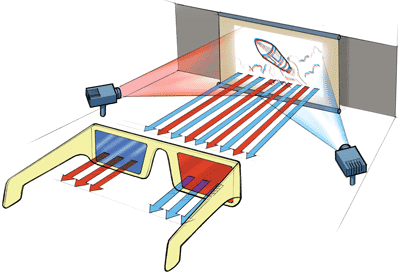
\includegraphics[width=250pt]{img/3d-glasses.png}
    \caption{3d polarized glasses}
    \label{fig:3d-glasses}
  \end{center}
\end{figure}
\\
Thanks to the robot double camera, two images from different point of
view are retrieved by the client (i.e. the teleoperator system) and
processed in order to recreate a 3D perspective, by one specific
technology (anaglyph stereo, polarized filter, HMD, and so on).
Figure \ref{fig:3d-glasses} shows an example with 3d polarized
glasses.
\\
The second approach was instead based on \textit{Augmented Reality}.
An augmented reality system generates a composite view for the user,
by combining the real scenes with virtual scenes generated by the
computer. In this way the scene is `augmented' with additional
information, enhancing operator's perception of the remote world.
\\
Information about depth perception, not available on
2D images, is recovered by laser sensor data. A laser scan sweeps the area
around the robot and returns distance values from near objects. Augmented
reality is used to mix information from camera and laser: starting from
stereo or mono pictures, information about distance is provided using colour
palette for making simple the perception of objects' proximity during
teleguide operation. A bundle of red lines is drawn starting from the robot
and ending in nearest objects' bases; for the further ones a bundle of green
lines is shown instead. In both case, it is possible to visualise the
exact distance from the object.
\\
More details can be found in \cite{morduc:macalusodetommaso}, while an
example is provided in figure \ref{fig:augmented_morduc}.
\begin{figure} [h]
  \begin{center}
    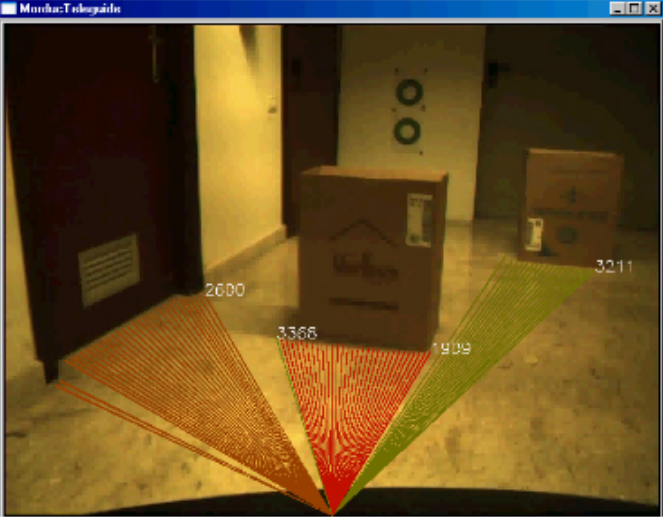
\includegraphics[width=250pt]{img/augmented_morduc.png}
    \caption{Client with Augmented Reality}
    \label{fig:augmented_morduc}
  \end{center}
\end{figure}
\\
A better perception of remote world can be achieved by other means,
for example by an \textit{exocentric} point of view. Next chapter
(\ref{intro:proposed_investigation}) will further explain this concept.



\begin{comment}
-- http://utminers.utep.edu/ydayal/aniko/index.html
-- http://en.wikipedia.org/wiki/Telerobotics
-- morduc:neri
-- morduc:macalusodetommaso
\end{comment}


%% EXOCENTRIC VISION

\section{The exocentric vision}
\subsection{Why exocentric vision ?}
\frame
{
  \frametitle{Why exocentric vision ?}
  
  \emph{It's difficult for an operator not accustomed to the vehicle
    to estimate the vehicle's position and direction and the distances to a target strictly
    based on camera images from the first person viewpoint\footnote{\tiny{as stated by M. Sugimoto and others}}.}
  \pause
  
  \vskip15pt

  \begin{block} {\alert{\texttt{Idea}}}
    An exocentric camera would provide a view of the robot in the operating
    environment and, thus, a better understanding of where the robot is located into the
    environment and its actual direction.
  \end{block}
  
  \pause
    
  \vskip5pt
  
  \begin{block} {\alert{\texttt{Trouble}}}
    Exocentric camera could be mounted on a rear-mounted protuberance of the robot,
    but such a protuberance would terribly limit the robot activity and its moving abilities.
  \end{block}
  
}

\frame
{
  \frametitle{Why exocentric vision ?}

  \begin{block} {\alert{\texttt{Solution}}}
    Simulate a virtual \textbf{exocentric} point of view, by drawing with augmented reality
    the robot on previous recorded first-person (i.e. \textbf{egocentric}) images, shot along its path. \\
    \pause
    Fixed a previous image put as \textbf{texture}, actual robot is drawn in order to
    simulate what a \textbf{rear} camera would shoot.  
  \end{block}

  %\vskip8pt
  \pause
  
  \begin{columns}
    
    \column{0.4\textwidth}
    \visible<3-> {
      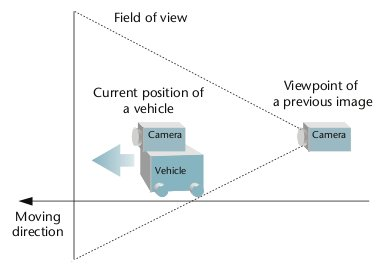
\includegraphics[width=\textwidth]{img/exocentric_vision.jpg}
    }

    \pause
    
    \column{0.2\textwidth}
    \visible<4-> {
      \begin{center}
        $\Longrightarrow$ \\
        \alert{virtual exocentric}
        \vskip4pt
        \scriptsize{(with augmented reality)}
      \end{center}
    }

    \pause

    \column{0.4\textwidth}
    \visible<5-> {
      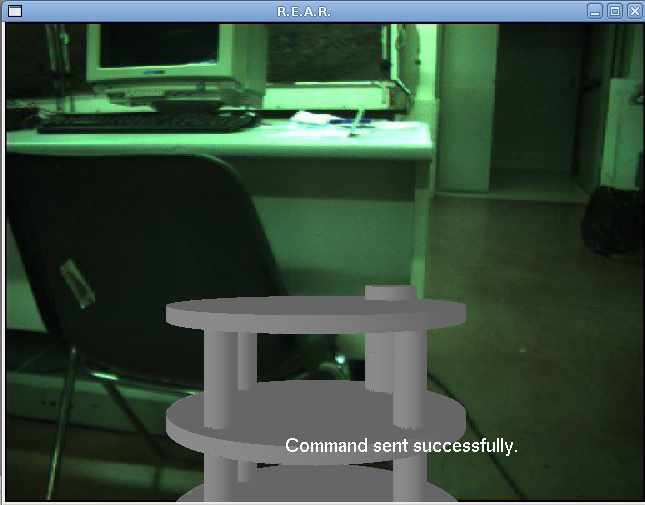
\includegraphics[width=\textwidth]{img/virtual_exocentric.png}
    }
    
  \end{columns}
  
  \pause
  
  \begin{block} {\alert{\texttt{Drawback}}}
    Environment must not change frequently.
  \end{block}


}

\subsection{Main issues}
\frame
{
  \frametitle{Main issues}


  
  \begin{block} {\alert{\texttt{We need to determinate}}}
    
    \pause
    
    \begin{itemize}
      
    \item \alert{\textit{how to draw the robot}} \\
      different robot must be drawn accordingly to
      their physic characteristics
      \pause
      
    \item \alert{\textit{how to choose the best image}} \\
      among all the egocentric images collected along
      its path, we need the one able to provide the most
      comprehensible external robot view
      \pause
      
    \item \alert{\textit{how to place the robot}} \\
      where to overlap a 3D robot representation      
    \end{itemize}
    
  \end{block}
}


%% REAR

\section{R.E.A.R.}
\subsection{Intro}
\frame
{
  \frametitle{Intro}
  
  \emph{\textit{R.E.A.R.} is a framework for the
    development of \textit{virtual exocentric vision systems}.}
  \pause
  
  \vskip15pt


  \begin{block} {\alert{\texttt{How it works}}}
    \begin{enumerate}

      \footnotesize

      \pause
      \item \texttt{take command input from user}
      \pause
      \item \texttt{send command to robot}
      \pause
      \item \texttt{retrieve robot position \& new egocentric image}
      \pause
      \item \texttt{add image to images' collection}
      \pause
      \item \texttt{choose the proper image to use as background}
      \pause
      \item \texttt{move the camera accordingly to the image chosen}
      \pause
      \item \texttt{move robot in its current position}
      
    \end{enumerate}
      
  \end{block}
      
}

\subsection{Independence from lower details}
\frame
{
  \frametitle{Independence from lower details}
  
  \emph{
    \textit{R.E.A.R.} exploits some object-oriented properties, such as \alert{polymorphism}
    and \alert{inheritance}, in order to work regardless of specific and low level details.
  }

  \vskip10pt
  \pause

  \begin{block} {\alert{\texttt{Lower details}}}
    \begin{itemize}

    \item \alert{\textit{how to draw the robot 3D model}} \\
      \pause

      \vskip5pt
      \only<3>{\footnotesize{user specifies a subclass of \alert{\texttt{Robot}} class: \\

          \begin{description} [\texttt{DrawRobot()}]

            \item [\texttt{DrawRobot()}]
              encapsulates how to draw the robot, through \textit{OpenGL} calls.

          \end{description}
        }}


      \pause

    \item \alert{\textit{how to choose the proper egocentric image}} \\
      \pause

      \vskip5pt
      \only<5>{\footnotesize{user specifies an implementation of \alert{\texttt{IImageSelector}} interface: \\

          \begin{description} [\texttt{ChoseImage()}]

            \item [\texttt{ChoseImage()}]
              encapsulates the exocentric image selection algorithm, given the current
              robot position and previous shot images' set.
          \end{description}
        }}
          
      \pause

    \item \alert{\textit{how to send and retrieve data to/from robot}} \\

      \pause
      \vskip5pt
      \only<7>{\footnotesize{user specifies an implementation of \alert{\texttt{IDataLogic}} interface: \\

          \begin{description} [\texttt{RetrieveData()}]
            \item [\texttt{SelectImage()}]
              delegates exocentric image selection to proper object; 
            \item [\texttt{RetrieveData()}]
              encapsulates how to read new status (i.e. position and egocentric
              image) from robot;
            \item [\texttt{Command()}]
              encapsulates how to send a movement command (forward, backward,
              left, right) to robot.
          \end{description}
        }}

      \pause

    \end{itemize}
    
  \end{block}
}


%% CONCRETE EXAMPLE

\section{Exocentric vision for 3m.o.r.d.u.c.}
\subsection{How to draw the robot}
\frame
{
  \frametitle{How to draw the robot}
  
  \emph{An exocentric vision system for \textit{3m.o.r.d.u.c.} 
    needs to tell \textit{R.E.A.R.} how to draw the robot itself,
    by subclassing \textbf{Robot} class.}
  \pause

  \vskip15pt

  \begin{block} {\alert{\texttt{Concrete classes}}}

    \pause
    \begin{itemize}
      
    \item \alert{\textit{Morduc}} \\
      3m.o.r.d.u.c. 3D model in \textit{OpenGL}
      \visible<3>{
        \begin{center}
          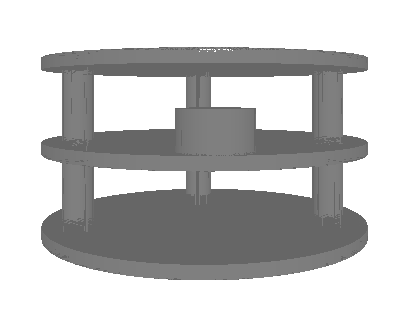
\includegraphics[width=80pt]{img/3morduc_opengl.png}
        \end{center}
      }
    \end{itemize}

  \end{block}
}

\subsection{How to choose the proper egocentric image}
\frame
{
  \frametitle{How to choose the proper egocentric image}
  
  \emph{An exocentric vision system for \textit{3m.o.r.d.u.c.} 
    needs to tell \textit{R.E.A.R.} how to choose the proper egocentric image,
    by implementig the \textbf{IImageSelector} interface.}
  \pause

  \vskip15pt

  \begin{block} {\alert{\texttt{Concrete classes}}}

    \begin{itemize}
      
    \pause
    \item \alert{\textit{SpacialMetricCalc}}
    \pause
    \item \alert{\textit{SweepMetricCalc}} \\
      details in next slide
    \pause
    \item \alert{\textit{AnotherSweepMetricCalc}} \\
      improvements of previous one, in order to
      provide user with more confortable teleguiding
      in case of strict turns

    \end{itemize}

  \end{block}
}

\subsubsection{Sweep Metric Algorithm}
\frame
{
  \frametitle{Sweep Metric Algorithm}
  
  \emph{Algorithm to choose the proper \textit{exocentric} image,
    among those collected.}
  \pause

  \begin{block} {\alert{\texttt{How it works}}}
 

    \begin{columns}
      
      \column{0.7\textwidth} {   
        \visible<2->{
          \begin{center}
            \only<2>{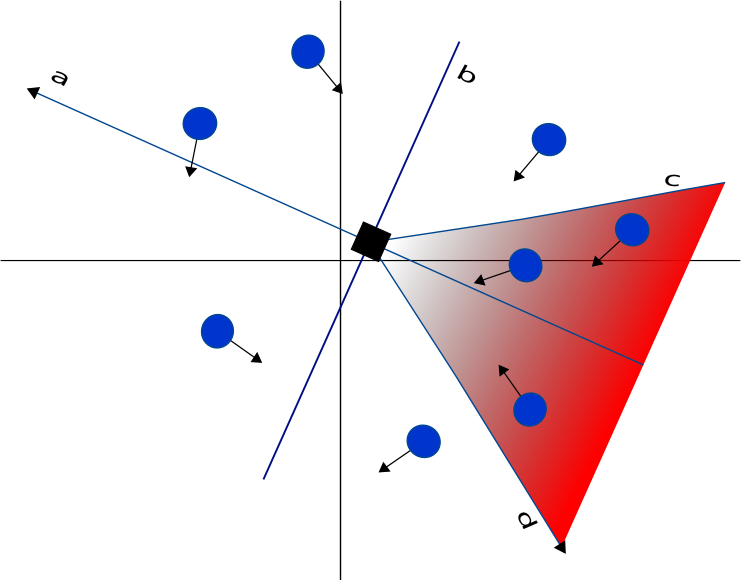
\includegraphics[width=0.8\textwidth]{img/sma_1.png}}
            \only<3>{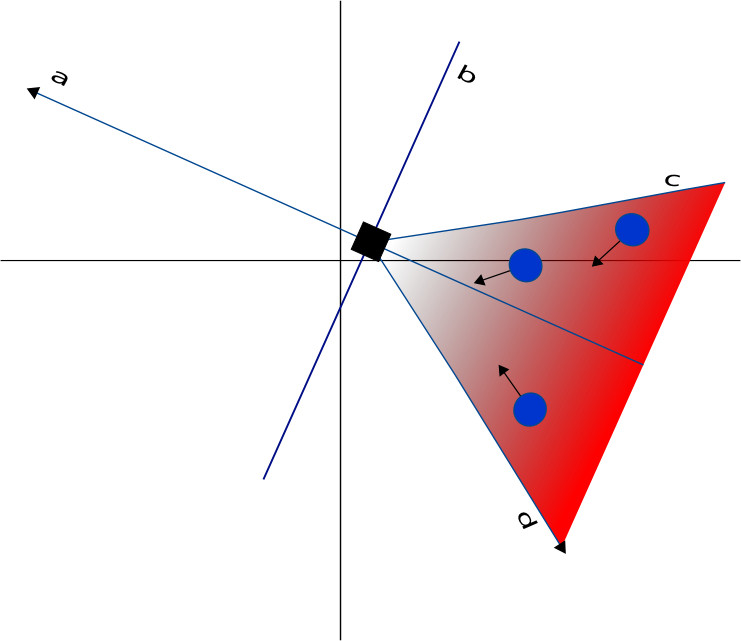
\includegraphics[width=0.8\textwidth]{img/sma_2.png}}
            \only<4>{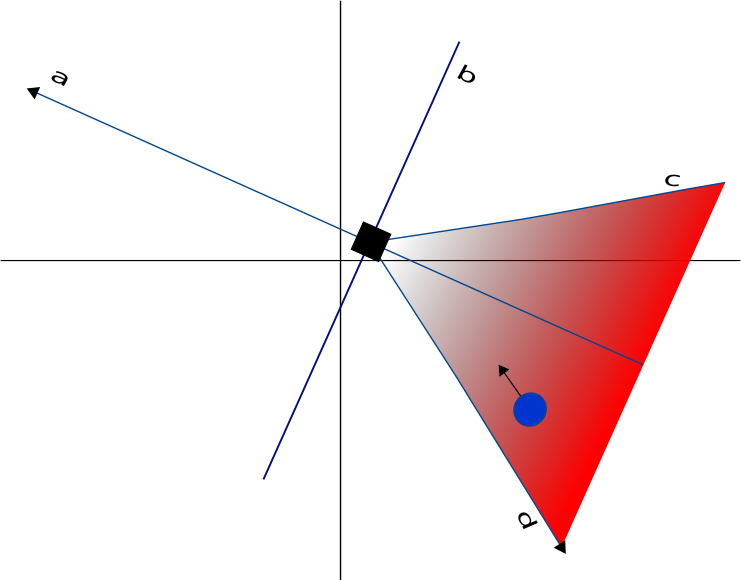
\includegraphics[width=0.8\textwidth]{img/sma_3.png}}
          \end{center}
        }
      }
      
      \column{0.2\textwidth} {
        \visible<2->{
          
          \scriptsize{Robot and image shot on XY plane}
          \vskip5pt
          
\includegraphics[width=8pt]{img/robot_icon.png} \\ 
          \tiny{robot oriented along sense indicated by line \textit{a}}
          \vskip5pt
          
\includegraphics[width=10pt]{img/image_icon.png} \\
          \tiny{image oriented along direction indicated by its arrow}
          \vskip5pt
          \tiny{red area indicates the \alert{\textit{sweep area}}}

        }
      }
      
    \end{columns}

    \vskip8pt
    
    \footnotesize{
      \only<2> {\alert{Step 0}: information about current robot position and image set are
      available.}
      \only<3> {\alert{Step 1}: discard all image shot outside the \textit{sweep area}.}
      \only<4> {\alert{Step 2}: discard all image shot with an orientation that differ more
        than a threadshold value from robot's orientation.}
     
    }
  \end{block}
}

\frame
{
  \frametitle{Sweep Metric Algorithm}
  
  \emph{Algorithm to choose the proper \textit{exocentric} image,
    among those collected.}

  \begin{block} {\alert{\texttt{How it works}}}
 
    At the end, three possible cases:
    \pause
    \begin{itemize}
      
    \item \alert{\textit{no images in \textit{sweep area}}} \\
      the egocentric image will be chosen
      \pause
      
    \item \alert{\textit{one image in \textit{sweep area}}} \\
      the unique image will be selected for exocentric vision
      \pause
      
    \item \alert{\textit{more than one image in \textit{sweep area}}} \\
      the image closer to an \textit{optimal distance} from the robot
      and with an orientation similar to robot's direction is chosen

      
    \end{itemize}
    
  \end{block}
}




\subsection{How to send and retrieve data to/from robot}
\frame
{
  \frametitle{How to send and retrieve data to/from robot}
  
  \emph{An exocentric vision system for \textit{3m.o.r.d.u.c.} 
    needs to tell \textit{R.E.A.R.} how to send and retrieve data to/from robot,
    by implementig the \textbf{IDataLogic} interface.}
  \pause

  \begin{block} {\alert{\texttt{Concrete classes}}}

    \begin{itemize}
      
    \pause
    \item \alert{\textit{DataLogicLogSimulator}} \\
      \footnotesize{
        new data are retrieved from log file written through
        a simulator session; acting
        in \textit{off-line} mode.
        }
    \pause
    \item \alert{\textit{DataLogicLogMorduc}} \\
      \footnotesize{
        new data are retrieved from log file written through
        a previous on-line teleguiding run accomplished with
        \textit{3m.o.r.d.u.c.}; acting
        in \textit{off-line} mode.
      }
    \pause
    \item \alert{\textit{DataLogicMorduc}} \\
      \footnotesize{
        new data and teleoperator's command are trasmitted from/to real 
        \textit{3m.o.r.d.u.c.}, through HTTP protocol; acting in
        \textit{on-line} mode.
      }
    \end{itemize}

  \end{block}
}


\subsection{Exocentric vs egocentric point of view}
\frame
{
  \frametitle{Exocentric vs egocentric point of view}
  
  \emph{Comparison between teleguiding \textit{3m.o.r.d.u.c.}
    form an egocentric and an exocentric point of view
    \footnote{\tiny{session recorded at DIIES laboratory}}.}
  \pause

  \begin{block} {\alert{\texttt{Teleoperator control}}}

    \begin{columns}
      
      \column{0.5\textwidth} {   
        \visible<2->{
          \footnotesize{Egocentric POV:}
          \begin{center}
            \only<2>{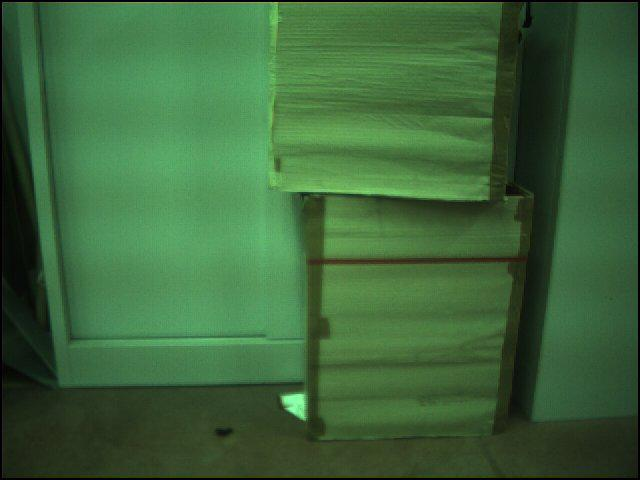
\includegraphics[width=0.9\textwidth]{img/log/img1.jpg}}
          \end{center}
        }
      }

      \column{0.5\textwidth} {   
        \visible<2->{
          \footnotesize{Exocentric POV:}
          \begin{center}
            \only<2>{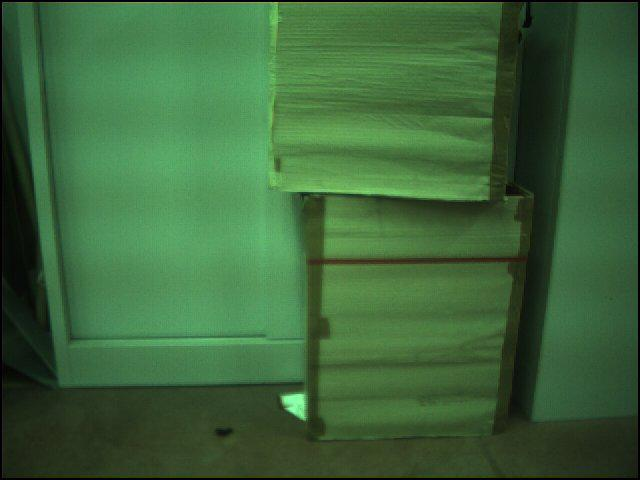
\includegraphics[width=0.9\textwidth]{img/log/img1.jpg}}
          \end{center}
        }
      }

    \end{columns}

    \vskip20pt
    
    \only<2>{Next command: \alert{go forward}}

  \end{block}
}


%% CONCLUSION

\section{Conclusion}
\frame
{
  \frametitle{Conclusion}
  
  \emph{Thank You For Paying Attention !}

  \vskip15pt

  For more information visit \\
  \vskip5pt
  \url{http://code.google.com/p/3morduc/}
  
}


\end{document}
